\documentclass[12pt,fleqn]{article}\usepackage{../../common}
\begin{document}
Yükseklik Fonksiyonu (Tepeler) Arasından En Düz, Optimal Yürüyüş Yolunu Bulmak

Elimizde bir alan içindeki yükseklikleri veren bir fonksiyon $f(x,y)$
olduğunu düşünelim. Acaba verili bir başlangıç ve bitiş noktası arasındaki
en ``rahat'' gidiş yolunu nasıl buluruz? 

Yükseklikler bir $E(x,y)$ fonksiyonunda olsun. Yolları nasıl temsil ederiz?
Bir parametrik eğri kullanabiliriz, mesela 

$$
x(t) = a_0 + a_1 t + a_2 t^2 + a_3 t^3 + a_4 t^4
$$

$$
y(t) = b_0 + b_1 t + b_2 t^2 + b_3 t^3 + b_4 t^4
$$

İstediğimiz derecede polinom parametrize eğrileri nasıl yaratacağımızı
biliyoruz [3]. Böylece doğru, optimal bir yolu bulmak demek
$a_0,a_1,a_2,a_3,b_0,b_1,b_2,b_3$ katsayılarını doğru bulmak demek
olacaktır. Bir optimizasyon problemi yani.

Peki o zaman optimize, minimize edilecek bedel fonksiyonu ne olmalı? Burada
farklı yaklaşımlar olabilir. Kimisi eğri altına düşen yüksekliklerin
toplamını bir çizgi entegrali ile hesaplamak isteyebilir. Fakat bu yaklaşım
yüksekliklerden genel olarak uzak dursa da mesela çok inişli çıkışlı
yolları hala tercih eder, ama bu tür yolların yürüyüş olarak yorucu
olacağını biliyoruz. 1000 metrelik bir tepeye çıkıp onun üzerinde düz
yürümek habire 1000 metreyi inmek çıkmaktan çok daha rahat.

Şu şekilde bir bedel belki daha iyi; Bir eğriyi düşünelim, onun $z$
eksenindeki yansıması da bir eğridir, $x,y$ düzlemindeki yansıması bir
başka eğri. Bu eğrilerin {\em uzunluğunu} hesaplarsak [2] ve dikey yöndeki
uzunluğu yatay olan uzunluğu farklı ağırlıklarla çarpıp toplarsak bu bir
bedeli temsil eder. Ağırlık dikey/yatay uzunluklar için 5/1 oranında
olabilir, o zaman yatay yöndeki bir uzunluk / katedilen yol dikeye göre 5
kat daha tercih edilir olur.

Önce yükseklikleri ve eğrileri iki örnek üzerinde görelim. Bir rasgele
tepe, ve bir rasgele yol çiziyoruz,

\begin{minted}[fontsize=\footnotesize]{python}
from mpl_toolkits.mplot3d import Axes3D
from scipy.spatial.distance import cdist
from matplotlib import cm

def gfunc(x, y):
    s1 = 2.2; x1 = 2.0; y1 = 2.0
    g1 = np.exp( -4 *np.log(2) * ((x-x1)**2+(y-y1)**2) / s1**2)
    return g1 * 10.0

def plot_surf_path(a0,a1,a2,a3,a4,b0,b1,b2,b3,b4):

    D = 50
    x = np.linspace(0,5,D)
    y = np.linspace(0,5,D)
    xx,yy = np.meshgrid(x,y)
    zz = gfunc(xx,yy)

    fig = plt.figure()
    ax = fig.gca(projection='3d')
    ax.set_xlim(0,5)
    ax.set_ylim(0,5)
    surf = ax.plot_wireframe(xx, yy, zz,rstride=10, cstride=10)

    t = np.linspace(0,1.0,100)

    x = a0 + a1*t + a2*t**2 + a3*t**3 + a4*t**4 
    y = b0 + b1*t + b2*t**2 + b3*t**3 + b4*t**4

    ax.plot3D(x, y, gfunc(x,y),'r.')
\end{minted}

\begin{minted}[fontsize=\footnotesize]{python}
# 1. gidis yolunun tanimi, uzun yoldan dolanarak gidiyor
a1,a2,a3 = 1.5, 8.1, 4.0
b1,b2,b3 = 0.3, 0.4, 23.3
a0,b0=(1.0,1.0)
ex,ey=(0.3,4.0)
a4 = ex - a0 - (a1+a2+a3)
b4 = ey - b0 - (b1+b2+b3)
test_coefs1 = (a0,a1,a2,a3,a4,b0,b1,b2,b3,b4)
plot_surf_path(a0,a1,a2,a3,a4,b0,b1,b2,b3,b4)

plt.savefig('calc_multi_40_elev_01.png')
\end{minted}


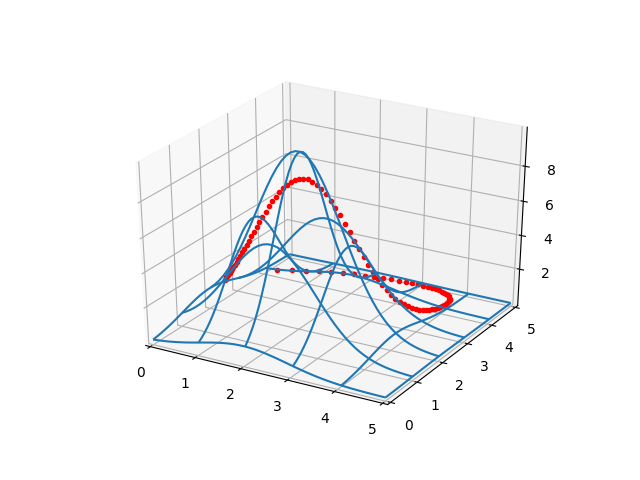
\includegraphics[width=20em]{calc_multi_40_elev_01.png}

Başlangıç ve bitiş noktalarını nasıl formüle dahil ettiğimize dikkat, $t=0$
olduğu anda $x(t),y(t)$ değerleri sırasıyla $a_0$ ve $b_0$'dir bunlar başlangıç
değerleridir. Bitiş noktası ise $t=1$ anında sahip olunması gereken değerdir,
bu noktada

$$
x(1) = a_0 + a_1 + a_2 + a_3 + a_4 ,\quad
y(1) = b_0 + b_1 + b_2 + b_3 + b_4 
$$

olacağı için bitiş noktalarına $e_x,e_y$ diyelim, $x(t)$ için $a_1,a_2,a_3$
katsayılarının değişmesine izin veririz, fakat sonuncu katsayı $a_4$'un ne
olacağını formülde $e_x$ üzerinden zorlarız, yani $a_4 = e_x - (a_0 + a_1 + a_2
+ a_3)$ hesabını yaparız. Böylece $a_0 + a_1 + a_2 + a_3 + a_4$ toplamı
$e_x$ sonucunu vermelidir. $y(t)$ ve $e_y$ için benzer mantığı kullanırız.

Eğer üstteki gidiş yoluna kuşbakışı, iki boyutlu ortamda bakmak istersek,

\begin{minted}[fontsize=\footnotesize]{python}
t = np.linspace(0,1.0,100)
x = a0 + a1*t + a2*t**2 + a3*t**3 + a4*t**4 
y = b0 + b1*t + b2*t**2 + b3*t**3 + b4*t**4
plt.xlim(0,5.0)
plt.ylim(0,5.0)
plt.plot(x,y)
plt.savefig('calc_multi_40_elev_02.png')
\end{minted}

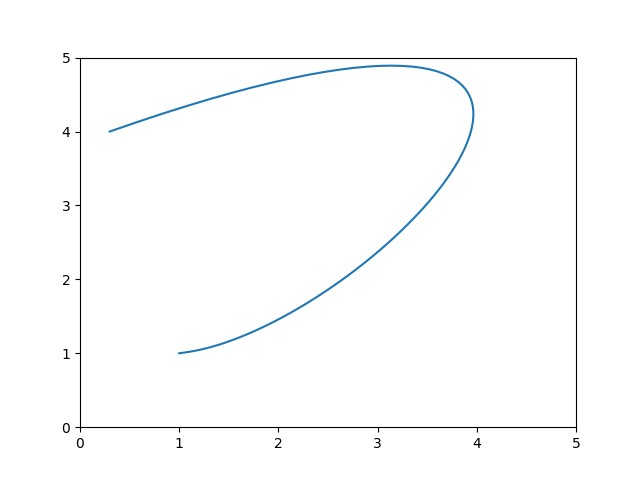
\includegraphics[width=20em]{calc_multi_40_elev_02.png}

Bu biraz önce bahsettiğimiz yatay düzlemdeki yansıma.

Şimdi ikinci bir gidiş yoluna bakalım, başlangıç noktası aynı ama bitiş farklı,

\begin{minted}[fontsize=\footnotesize]{python}
# 2. gidis yolunun tanimi, dik cikip iniyor
a1,a2,a3 = 1.5, 3.0, 1.0
b1,b2,b3 = 0.0, 1.0, 1.0
a0,b0=(1.0,1.0)
ex,ey=(0.3,4.0)
a4 = ex - a0 - (a1+a2+a3)
b4 = ey - b0 - (b1+b2+b3)
test_coefs2 = (a0,a1,a2,a3,a4,b0,b1,b2,b3,b4)
plot_surf_path(a0,a1,a2,a3,a4,b0,b1,b2,b3,b4)
plt.savefig('calc_multi_40_elev_03.png')
\end{minted}

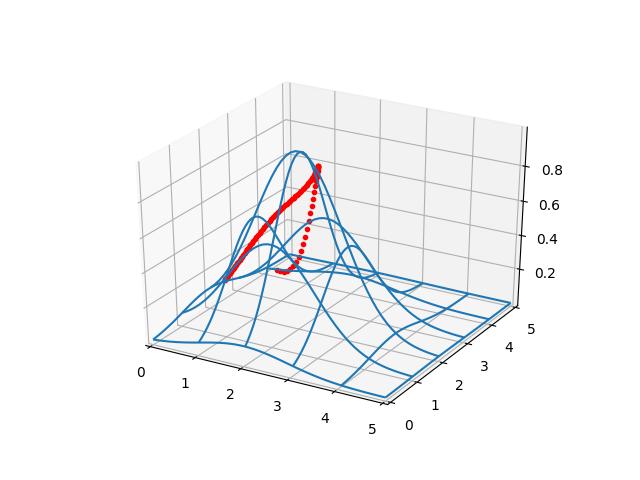
\includegraphics[width=20em]{calc_multi_40_elev_03.png}

Bu yolları tabii ki rasgele parametreler üzerinden yarattık, bunlar optimal
yollar değiller.

Optimallik için gereken uzunluk hesabına gelelim. Bu hesap için
formül, dikey için $I_v$ yatay için $I_h$

$$
I_v = \int_{t=0}^{t=1} \sqrt{1 + \left(\frac{\ud z}{\ud t} \right)^2 } \ud t
$$

$$
I_h = \int_{t=0}^{t=1} \sqrt{
\left(\frac{\ud x}{\ud t} \right)^2 + 
\left(\frac{\ud y}{\ud t} \right)^2
} 
\ud t
$$


Formülde görülen $\ud z/\ud t$, $\ud x/\ud t$ ve $\ud y/\ud t$, parametrik eğri
üzerinden alınacak tabii ki. Problem çözümü açısından $\ud z/\ud t$ hesabı
külfetli olabilir, çünkü $z = f(x,y)$ yükseklik fonksiyonundur. Üstteki
örnekteki yükseklik fonksiyonu basit, ama daha çetrefil durumlarda da
kullanabileceğimiz bir yaklaşım daha iyi olur. Bu sebeple $\ud z/\ud t$ türevini
hesapsal yapacağız.

Ama yatay türevler $\ud x/\ud t$ ve $\ud y/\ud t$ için, türevi almak, kare,
toplam, karekök hesaplarını sembolik olarak yapabiliriz, çünkü bu formül
polinom, formu şimdiden belli.

\begin{minted}[fontsize=\footnotesize]{python}
import sympy

vars = 't a0 a1 a2 a3 b0 b1 b2 b3 gamma x y'
t, a0, a1, a2, a3, b0, b1, b2, b3, gamma, x, y = sympy.symbols(vars)

xdef = a0 + a1*t + a2*t**2 + a3*t**3 + a4*t**4
ydef = b0 + b1*t + b2*t**2 + b3*t**3 + b4*t**4

dxdt = sympy.diff(xdef,t)
print (dxdt)
dydt = sympy.diff(ydef,t)
print (dydt)
sqrtdef = sympy.sqrt(sympy.diff(xdef,t)**2 + sympy.diff(ydef,t))
print (sqrtdef)
\end{minted}

\begin{verbatim}
a1 + 2*a2*t + 3*a3*t**2 - 57.2*t**3
b1 + 2*b2*t + 3*b3*t**2 - 84.0*t**3
sqrt(b1 + 2*b2*t + 3*b3*t**2 - 84.0*t**3 + (a1 + 2*a2*t + 3*a3*t**2 - 57.2*t**3)**2)
\end{verbatim}

Entegraller $I_v,I_h$ hesapları da sayısal yapılacak.

Hepsini bir araya koyarsak, uzunluklar (entegraller) üzerinden bir bedel
elde ediyoruz, ve bu bedeli minimize edecek eğri parametrelerini bulmak
için ise optimizasyon işletiyoruz. Optimizasyon kısıtlamalar içerecek, eğri
parametrelerinin -5/+5 arasında olmasını istiyoruz mesela.

\begin{minted}[fontsize=\footnotesize]{python}
from scipy.optimize import minimize, Bounds, SR1, BFGS
import numpy as np
import matplotlib.pyplot as plt
from mpl_toolkits.mplot3d import Axes3D
from scipy.spatial.distance import cdist
from matplotlib import cm
import util

def trapz(y, dx):
    vals = y[1:-1]
    vals = vals[vals>0.0]
    return (y[0]+np.sum(vals*2.0)+y[-1])*(dx/2.0)


def find_path(ex,ey,a0,b0):
    
    def calc_int(pars):
        a1,a2,a3,b1,b2,b3=pars
        a4 = ex - a0 - (a1+a2+a3)
        b4 = ey - b0 - (b1+b2+b3)
        def gfunc(t):
            t = t[0]
            x = a0 + a1*t + a2*t**2 + a3*t**3 + a4*t**4 
            y = b0 + b1*t + b2*t**2 + b3*t**3 + b4*t**4
            s1 = 2.2; x1 = 2.0; y1 = 2.0
            g1 = np.exp( -4 *np.log(2) * ((x-x1)**2+(y-y1)**2) / s1**2)
            return g1*10.0    
        ts = np.linspace(0.0,1.0,100)
        dzs = np.array([util._approx_fprime_helper([t],gfunc)[0] for t in ts])
        tmp = np.sqrt(1.0+(dzs**2.0))
        Iv = trapz(tmp, 1/100.)
        tmp = np.array([b1 + 2*b2*t + 3*b3*t**2 - 112.0*t**3 + (a1 + 2*a2*t + 3*a3*t**2 - 65.2*t**3)**2 for t in ts])
        tmp = tmp[tmp>0.0]
        tmp = np.sqrt(tmp)
        Ih = trapz(tmp, 1/100.)
        res = Iv*5 + Ih*1
        return res 
    
    LIM = 5.0
    # rasgele secilmis baslangic degerleri
    a1,a2,a3 = 0,0,0
    b1,b2,b3 = 0,0,0
    x0 = a1,a2,a3,b1,b2,b3

    opts = {'maxiter': 300, 'verbose': 0}
    res = minimize (fun=calc_int,
                    x0=x0,
                    method='trust-constr',
                    hess = BFGS (),
                    bounds=Bounds([-LIM, -LIM, -LIM, -LIM, -LIM, -LIM],
                                  [LIM, LIM, LIM, LIM, LIM, LIM]),
                    options=opts)
    

    return res

a0,b0=(1.0,1.0)
ex,ey=(0.3,4.0)
res = find_path(ex,ey,a0,b0)
print  ('res',res)
print  ('res',res['x'])

a0,b0=(4.0,1.0)
ex,ey=(1.0,4.0)
res = find_path(ex,ey,a0,b0)
print  ('res',res)
print  ('res',res['x'])
\end{minted}

\begin{verbatim}
res  barrier_parameter: 6.400000000000003e-06
 barrier_tolerance: 6.400000000000003e-06
          cg_niter: 1604
      cg_stop_cond: 2
            constr: [array([-1.08548354, -0.36789632, -0.20897387,  0.2395503 ,  0.29868552,
        0.00380265])]
       constr_nfev: [0]
       constr_nhev: [0]
       constr_njev: [0]
    constr_penalty: 1.0
  constr_violation: 0.0
    execution_time: 50.29004144668579
               fun: 33.11613644482912
              grad: array([-1.38273935, -0.50301313,  0.79182863,  1.80994987,  2.2042923 ,
        2.09085321])
               jac: [<6x6 sparse matrix of type '<class 'numpy.float64'>'
	with 6 stored elements in Compressed Sparse Row format>]
   lagrangian_grad: array([-1.2659412 , -0.46518832,  0.73288924,  1.67502195,  2.03938462,
        1.93597495])
           message: 'The maximum number of function evaluations is exceeded.'
            method: 'tr_interior_point'
              nfev: 2723
              nhev: 0
               nit: 301
             niter: 301
              njev: 0
        optimality: 2.0393846199040575
            status: 0
           success: False
         tr_radius: 1.8588829764195948e-08
                 v: [array([ 0.11679815,  0.03782481, -0.05893939, -0.13492793, -0.16490768,
       -0.15487826])]
                 x: array([-1.08548354, -0.36789632, -0.20897387,  0.2395503 ,  0.29868552,
        0.00380265])
res [-1.08548354 -0.36789632 -0.20897387  0.2395503   0.29868552  0.00380265]
...
res [-0.3061632   4.76223126  4.99872105  0.41013189  4.9713953   4.9745472 ]
\end{verbatim}

Bir optimal sonuç bulundu. Grafikleyelim,

\begin{minted}[fontsize=\footnotesize]{python}
a1,a2,a3,b1,b2,b3 = -1.08548354, -0.36789632, -0.20897387,  0.2395503,   0.29868552,  0.00380265
a4 = ex - a0 - (a1+a2+a3)
b4 = ey - b0 - (b1+b2+b3)
plot_surf_path(a0,a1,a2,a3,a4,b0,b1,b2,b3,b4)
plt.savefig('calc_multi_40_elev_04.png')
\end{minted}

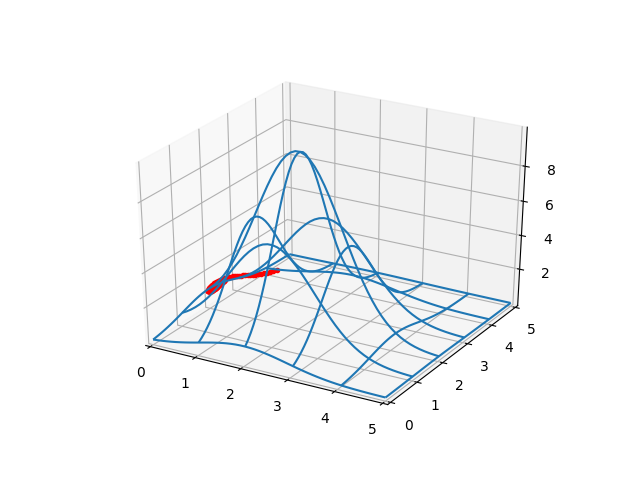
\includegraphics[width=20em]{calc_multi_40_elev_04.png}

Yol oldukca optimal duruyor. Gereksiz iniş çıkış yok, ve yatay mesafe de
minimize edilmiş. 

İkinci örnek 

\begin{minted}[fontsize=\footnotesize]{python}
a0,b0=(4.0,1.0)
ex,ey=(1.0,4.0)
a1,a2,a3,b1,b2,b3 = -0.3061632,   4.76223126,  4.99872105,  0.41013189,  4.9713953,   4.9745472 
a4 = ex - a0 - (a1+a2+a3)
b4 = ey - b0 - (b1+b2+b3)
plot_surf_path(a0,a1,a2,a3,a4,b0,b1,b2,b3,b4)
plt.savefig('calc_multi_40_elev_05.png')
\end{minted}

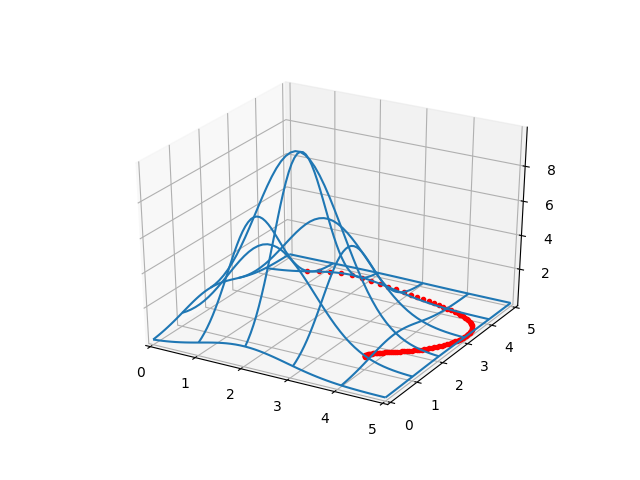
\includegraphics[width=20em]{calc_multi_40_elev_05.png}

Görüldüğü gibi yol tepeden uzak durmaya uğraşmış.

Farklı Eğri Yöntemi ve Bitiş Noktası Sınırlaması

[3]'te alternatif bir eğri şekli daha gördük, lineer parçalı ya da sigmoid
bazlı parametrize eğriler. Bir parametrize eğriyi 

$$
x = a_0 + a_1 \sigma(t,u_1) + a_2 \sigma(t,u_2) + ... 
$$

$$
x = b_0 + b_1 \sigma(t,v_1) + b_2 \sigma(t,v_2) + ... 
$$

modelleyebilirdik, $u_1,u_2,..$ eksen $x$ için ilmik noktaları,
$v_1,v_2,..$ eksen $y$ için ilmik noktaları olabilirdi ve biraz
değiştirilmiş sigmoid $\sigma$ ifadesi

$$
\sigma (x,k) = (x-k) \frac{1}{1 + exp(-\alpha (x-k))}
$$

Bilindiği gibi normal sigmoid ifadesi

$$
\sigma (x) = \frac{1}{1 + exp(-\alpha x)}
$$

ve $\alpha$ büyüdükçe 0'dan 1'e geçiş sertleşir. 

Bu şekilde parametrize edilmiş eğri ile pek çok farklı şekil ortaya
çıkartılabilir. Bitiş noktasını da farklı bir şekilde optimizasyon kısıtlaması
üzerinden zorluyoruz [3].

\begin{minted}[fontsize=\footnotesize]{python}
from scipy.optimize import minimize, Bounds, SR1, BFGS
import numpy as np
import matplotlib.pyplot as plt
from mpl_toolkits.mplot3d import Axes3D
from matplotlib import cm
import util

rho = 7.0
def sig(x,a):
   return (x-a)*1/(1+np.exp(-rho*(x-a)))

def trapz(y, dx):
    vals = y[1:-1]
    vals = vals[vals>0.0]
    return (y[0]+np.sum(vals*2.0)+y[-1])*(dx/2.0)

def plot_surf_path(a0,a1,a2,a3,b0,b1,b2,b3):

    D = 50
    x = np.linspace(0,5,D)
    y = np.linspace(0,5,D)
    xx,yy = np.meshgrid(x,y)
    zz = gfunc(xx,yy)

    fig = plt.figure()
    ax = fig.gca(projection='3d')
    ax.set_xlim(0,5)
    ax.set_ylim(0,5)
    surf = ax.plot_wireframe(xx, yy, zz,rstride=10, cstride=10)

    t = np.linspace(0,5.0,100)

    def sigx(t):
        t = t[0]
        x = a0 + \
            a1*sig(t,1) + \
            a2*sig(t,2) + \
            a3*sig(t,3)
        return x
    
    def sigy(t):
        t = t[0]
        y = b0 + \
            b1*sig(t,1) + \
            b2*sig(t,2) + \
            b3*sig(t,3)
        return y


    xs = np.array([sigx([tt]) for tt in t])
    ys = np.array([sigy([tt]) for tt in t])
    
    ax.plot3D(xs, ys, gfunc(xs,ys),'r.')

 
def find_path(ex,ey,a0,b0):
    
    def calc_int(pars):
        a1,a2,a3,b1,b2,b3=pars
        def sigx(t):
            t = t[0]
            x = a0 + \
                a1*sig(t,1) + \
                a2*sig(t,2) + \
                a3*sig(t,3)
            return x
        
        def sigy(t):
            t = t[0]
            y = b0 + \
                b1*sig(t,1) + \
                b2*sig(t,2) + \
                b3*sig(t,3)
            return y
        
        def gfunc(t):
            t = t[0]
            x = sigx([t])	   
            y = sigy([t])
            s1 = 2.2; x1 = 2.0; y1 = 2.0
            g1 = np.exp( -4 *np.log(2) * ((x-x1)**2+(y-y1)**2) / s1**2)
            s2 = 1.2; x2 = 4.0; y2 = 1.0
            g2 = np.exp( -4 *np.log(2) * ((x-x2)**2+(y-y2)**2) / s2**2)
            return g1*10.0 + g2*10.0
         
        ts = np.linspace(0.0,5.0,100)
        dzs = np.array([util._approx_fprime_helper([t],gfunc)[0] for t in ts])
        tmp = np.sqrt(1.0+(dzs**2.0))
        Iv = trapz(tmp, 5./100)
        dxs = np.array([util._approx_fprime_helper([t],sigx)[0] for t in ts])
        dys = np.array([util._approx_fprime_helper([t],sigy)[0] for t in ts])
        tmp = np.power(dxs,2) + np.power(dys,2)
        tmp = tmp[tmp>0.0]
        tmp = np.sqrt(tmp)
        Ih = trapz(tmp, 5./100)
        res = Iv*5.0 + Ih*1.0
        #print (res)
        return res 
    
    LIM = 2.0

    a1,a2,a3,b1,b2,b3 = 0.1, 0.1, 0.1, 0.1, 0.1, 0.1
    x0 = a1,a2,a3,b1,b2,b3

    opts = {'maxiter': 50, 'verbose': 0}
    
    def conx(x):
        aa1,aa2,aa3,bb1,bb2,bb3 = x
        a = a0+aa1*(5.0-1.0)+aa2*(5.0-2.0)+aa3*(5.0-3.0)-ex
        return a
    
    def cony(x):
        aa1,aa2,aa3,bb1,bb2,bb3 = x
        b = b0+bb1*(5.0-1.0)+bb2*(5.0-2.0)+bb3*(5.0-3.0)-ey
        return b
    
    cons = [{'type':'eq', 'fun': conx}, {'type':'eq', 'fun': cony}]
    
    res = minimize (fun=calc_int,
                    x0=x0,
                    method='trust-constr',
                    hess = BFGS (),
                    bounds=Bounds([-LIM, -LIM, -LIM, -LIM, -LIM, -LIM],
                                  [ LIM,  LIM,  LIM,  LIM,  LIM,  LIM]),
                    constraints=cons,
                    options=opts)
    

    return res

a0,b0=(1.0,1.0)
ex,ey=(4.0,2.0)
res = find_path(ex,ey,a0,b0)
print  ('res',res)
print  ('res',res['x'])
\end{minted}

\begin{verbatim}
0.54188089  0.15991385  0.17636745 -0.20027426  0.26754927  0.4992246 
\end{verbatim}

\begin{minted}[fontsize=\footnotesize]{python}
import pandas as pd
import numpy as np
import matplotlib.pyplot as plt
from mpl_toolkits.mplot3d import Axes3D
from scipy.spatial.distance import cdist
from matplotlib import cm

rho = 7.0
def sig(x,a):
   return (x-a)*1/(1+np.exp(-rho*(x-a)))

def gfunc(x, y):
    s1 = 2.2; x1 = 2.0; y1 = 2.0
    g1 = np.exp( -4 *np.log(2) * ((x-x1)**2+(y-y1)**2) / s1**2)
    s2 = 1.2; x2 = 4.0; y2 = 1.0
    g2 = np.exp( -4 *np.log(2) * ((x-x2)**2+(y-y2)**2) / s2**2)
    return g1*10.0 + g2*10.0

def plot_surf_path(a0,a1,a2,a3,b0,b1,b2,b3):

    D = 50
    x = np.linspace(0,5,D)
    y = np.linspace(0,5,D)
    xx,yy = np.meshgrid(x,y)
    zz = gfunc(xx,yy)

    fig = plt.figure()
    ax = fig.gca(projection='3d')
    ax.set_xlim(0,5)
    ax.set_ylim(0,5)
    surf = ax.plot_wireframe(xx, yy, zz,rstride=10, cstride=10)

    t = np.linspace(0,5.0,100)

    def sigx(t):
        t = t[0]
        x = a0 + \
            a1*sig(t,1) + \
            a2*sig(t,2) + \
            a3*sig(t,3)
        return x
    
    def sigy(t):
        t = t[0]
        y = b0 + \
            b1*sig(t,1) + \
            b2*sig(t,2) + \
            b3*sig(t,3)
        return y


    xs = np.array([sigx([tt]) for tt in t])
    ys = np.array([sigy([tt]) for tt in t])

    ax.view_init(elev=45, azim=-113)
    ax.plot3D(xs, ys, gfunc(xs,ys),'r.')

a1,a2,a3,b1,b2,b3=0.54187919,  0.15991569,  0.17636809, -0.20027283,  0.26755009,  0.49922053
a0,b0=(1.0,1.0)
plot_surf_path(a0,a1,a2,a3,b0,b1,b2,b3)
#plt.show()
plt.savefig('calc_multi_40_elev_06.png')
# -113,45
\end{minted}

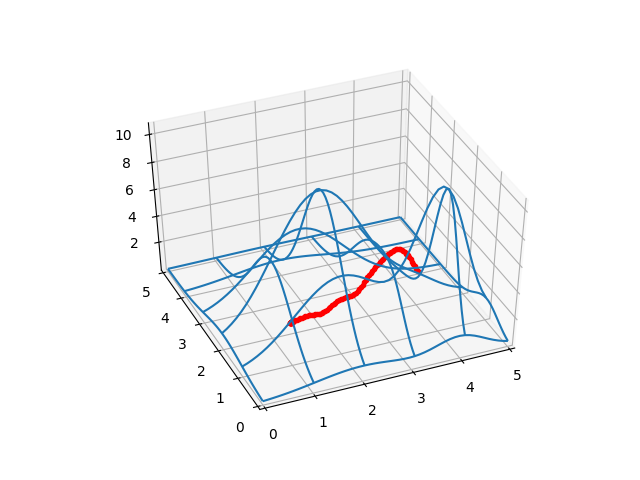
\includegraphics[width=20em]{calc_multi_40_elev_06.png}

Sadece 3 tane ilmik noktası tanımladık, bu noktalar vektörel notasyon ile
çoğaltılabilir. Fakat optimizasyon gayet optimal bir yolu bulabildi, bu
örnekte iki tane tepe var, ama onların arasından geçerek sonuca ulaştı. 

Bitiş noktalarını cebirsel değil \verb!conx! ve \verb!cony! adlı iki
sınırlama tabiri ile zorladık.

Polinom bazlı eğride bazı türevleri sembolik olarak almıştık, burada
tüm türevler sayısal bazlı fakat sigmoid bazlı parametrik eğrilerin de
sembolik türevini kullanmak zor değil. Burada hızlı kodlama amaçlı bunu
yapmadık. 

Kaynaklar 

[1] Bayramlı, Sayısal Bilim, {\em Sayısal Entegrasyon (Numerical Integration)}

[2] Bayramlı, Çok Boyutlu Calculus, {\em Ders 6, Eğri Uzunluğu}

[3] Bayramlı, Çok Boyutlu Calculus, {\em Ders 5, İki Nokta Arasında Parametrize Edilmiş Eğri}

[4] Bayramlı, İstatistik ve Veri Analizi, {\em Dairesel Baz Fonksiyonları (Radial Basis Functions -RBF-)}

[5] Bayramlı, Fonksiyonel Analiz ve Optimizasyon, {\em Newton-umsu Metotlar, DFP, BFGS }

\end{document}

